\documentclass[../TDE4-E5.tex]{subfiles}%

\begin{document}
\section[s]"1"{Masse percutant un ressort}

\enonce{%
	\noindent
	\begin{minipage}{0.70\linewidth}
		Un ressort (raideur $k$ et longueur à vide $\ell_0$) fixé en $O$ est
		initialement au repos. Une masse $m$ glisse sans frottement à vitesse
		constante $\vv{v} = -v_0\vv*{u}{x}$ avec $v_0 > 0$
		et s'accroche \textit{définitivement} au ressort à l'instant $t = 0$.
	\end{minipage}
	\hfill
	\begin{minipage}{0.3\linewidth}
		\centering
		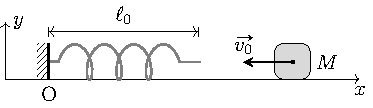
\includegraphics[width=\linewidth]{ressort_v0_plain}
	\end{minipage}
}%

\QR{%
	Déterminer l'équation du mouvement de la masse une fois qu'elle est
	accrochée (pour $t \geq 0$).
}{%
	Une fois la masse accrochée, on retrouve la
	situation du cours. On fait le bilan des forces~:
	\noindent
	\begin{minipage}[c]{.48\linewidth}
		\[
			\begin{array}{ll}
				\textbf{Poids}   & \Pf = -mg\uy                  \\
				\textbf{Support} & \Rf = R\uy                    \\
				\textbf{Ressort} & \Ff = -k(\ell(t) - \ell_0)\ux
			\end{array}
		\]
	\end{minipage}
	\hfill
	\begin{minipage}[c]{.48\linewidth}
		\begin{center}
			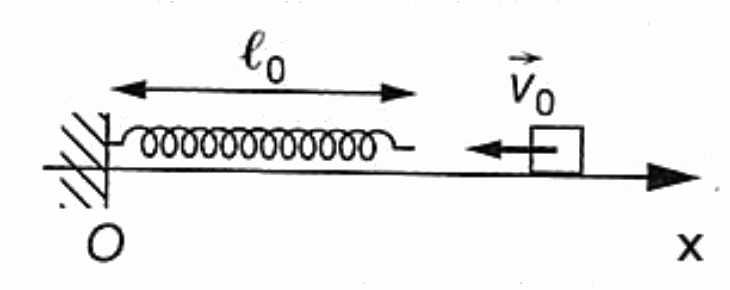
\includegraphics[width=\linewidth]{ressort_v0}
		\end{center}
	\end{minipage}
	On effectue le changement de variable $x(t) = \ell(t) -\ell_0$, et avec le PFD
	on a donc
	\begin{gather*}
		m\af = \Pf + \vv{R} + \Ff\\
		\Leftrightarrow m\left(
		\begin{array}{c}
				\DS\dv[2]{x}{t} \\
				0
			\end{array}
		\right)
		=
		\left(
		\begin{array}{c}
				-kx \\
				-mg + R
			\end{array}
		\right)
	\end{gather*}
	Sur l'axe $\ux$ on trouve bien
	\begin{equation*}
		\boxed{m \dv[2]{x}{t} + kx = 0}
		\Lra
		\boxed{\dv[2]{x}{t} + \w_0{}^2x = 0}
	\end{equation*}
	avec $\w_0 = \sqrt{\dfrac{k}{m}}$. La projection sur $\uy$ montre que la
	réaction du support compense le poids.
}

\QR{%
	Résoudre cette équation en tenant compte des conditions initiales.
}{%
	À $t=0$, la masse est accrochée au ressort de longueur $\ell_0$ et elle arrive
	avec $\vf(0) = -v_0\ux$. On a donc
	\begin{equation*}
		\boxed{x(0) = 0}
		\qet
		\boxed{\qty(\dv{x}{t})_{0} = -v_0}
	\end{equation*}
	La forme générale de la solution est
	\[ \boxed{x(t) = A\cos(\w_0t) + B\sin(\w_0t)}\]
	Avec conditions initiales,
	\begin{gather*}
		x(0) =
		A\underbracket[1pt]{\cos(0)}_{=1} + B\underbracket[1pt]{\sin(0)}_{=0}
		\Lra
		A = 0
		\\
		\qty(\dv{x}{t})_0 =
		-A\w_0\underbracket[1pt]{\sin(0)}_{=0} +
		B\w_0\underbracket[1pt]{\cos(0)}_{=1}
		\Lra
		B = - \frac{v_0}{\w_0}
	\end{gather*}
	On a donc
	\begin{equation*}
		\boxed{x(t) = -\frac{v_0}{\w_0}\sin(\w_0t)}
	\end{equation*}
}%

\QR{%
	À quelle condition la masse vient-elle percuter la paroi en O~?
}{%
	En supposant que le ressort puisse se comprimer à l'infini, la masse vient
	percuter la paroi située en $O$ si l'amplitude de $x(t)$ est égale à
	$-\ell_0$, c'est-à-dire
	\[\boxed{\frac{v_0}{\w_0} = \ell_0} \Leftrightarrow \boxed{v_0 = \w_0\ell_0}\]
	On remarque donc que plus $v_0$ est grande, plus cela est facile, mais
	également que plus $\w_0$ est faible est plus cela est facile. En effet, plus
	la pulsation est élevée et moins la masse a d'amplitude à $v_0$ fixée. Ceci
	correspond bien à l'intuition qu'on pourrait en avoir énergétiquement~: une
	énergie mécanique totale se répartit dans l'énergie potentielle élastique
	d'une part, c'est-à-dire la distance d'élongation du ressort, et dans
	l'énergie cinétique d'autre part, donc dans sa vitesse.
}

\end{document}
